%% query_cost.tex — Theoretical vs measured query counts
%% Data from benchmark run 2026-04-09

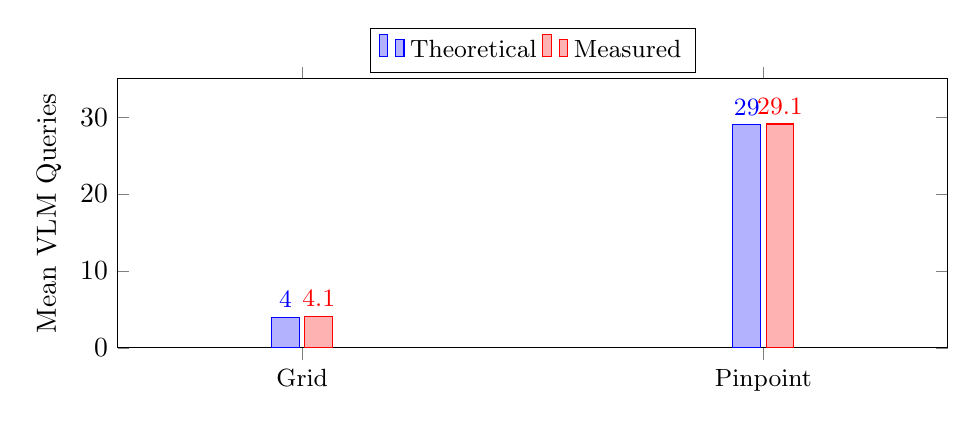
\begin{tikzpicture}
\begin{axis}[
    ybar,
    bar width=10pt,
    width=\columnwidth,
    height=5cm,
    ylabel={Mean VLM Queries},
    symbolic x coords={Grid, Pinpoint},
    xtick=data,
    xticklabel style={font=\small},
    ymin=0, ymax=35,
    legend style={
      at={(0.5,1.02)}, anchor=south,
      legend columns=2, font=\small,
    },
    nodes near coords,
    nodes near coords style={font=\small},
    enlarge x limits=0.4,
  ]

  % Theoretical: Grid=4 (2 axes x 2 iterations), Pinpoint=4+1+24=29
  \addplot coordinates {
    (Grid, 4) (Pinpoint, 29)
  };

  % Measured average
  \addplot coordinates {
    (Grid, 4.1) (Pinpoint, 29.1)
  };

  \legend{Theoretical, Measured}

\end{axis}
\end{tikzpicture}
